\documentclass{scrartcl}

\usepackage[utf8]{inputenc} % Unicode support (Umlauts etc.)
\usepackage{hyperref} % Add a link to your document
\usepackage{graphicx} % Add pictures to your document
\usepackage{listings} % Source code formatting and highlighting
\usepackage{algpseudocode}
\usepackage[top=75px, bottom=75px, left=85px, right=85px]{geometry} % Change page borders
\usepackage{enumitem}
\usepackage{algpseudocode}
\usepackage{mathtools}
\usepackage{fancyhdr}
\usepackage{framed}
\usepackage{amsmath, amssymb, graphics, setspace} 
\pagestyle{fancy}
\fancyhead{}
\fancyfoot[R]{Data Mining: Assignment 3}
\fancyfoot[L]{Tom Harting}
\renewcommand{\headrulewidth}{0pt}
\renewcommand{\footrulewidth}{0.4pt}

\begin{document}

\title{Data Mining}
\subtitle{Assignment 3}
\date{\today{}}

\author{
    \begin{tabular}{l r}
        Tom Harting & 4288319 \\
        Sven Popping & 4289455 \\
    \end{tabular}
}

\maketitle \pagebreak

\begin{enumerate}
	\item Please see Appendix figure \ref{fig:g1}.
	\item $\begin{bmatrix}
		0 & 0 & 1 & 0 \\
		\frac{1}{3} & 0 & 0 & \frac{1}{2} \\
		\frac{1}{3} & 0 & 0 & \frac{1}{2} \\
		\frac{1}{3} & 1 & 0 & 0 \\
	\end{bmatrix}$
	\item $\begin{bmatrix}
		\frac{1}{4} \\
		\frac{5}{24} \\
		\frac{5}{24} \\
		\frac{1}{3} \\
	\end{bmatrix}$
	\item There are no outgoing edges to A, therefor it's value is 0. C only has an outgoing edge to itself, therefor it's value is almost 1 (if you go from A, B or D to C you can't leave C).
	\item Yes they are, the value of A is still low, cause you can only reach A via the teleport. The value of C is still high because there is stil l a change that it keeps linking to itself without teleporting.
\end{enumerate}

\pagebreak
\section*{Appendix}
\begin{figure}[h!]
	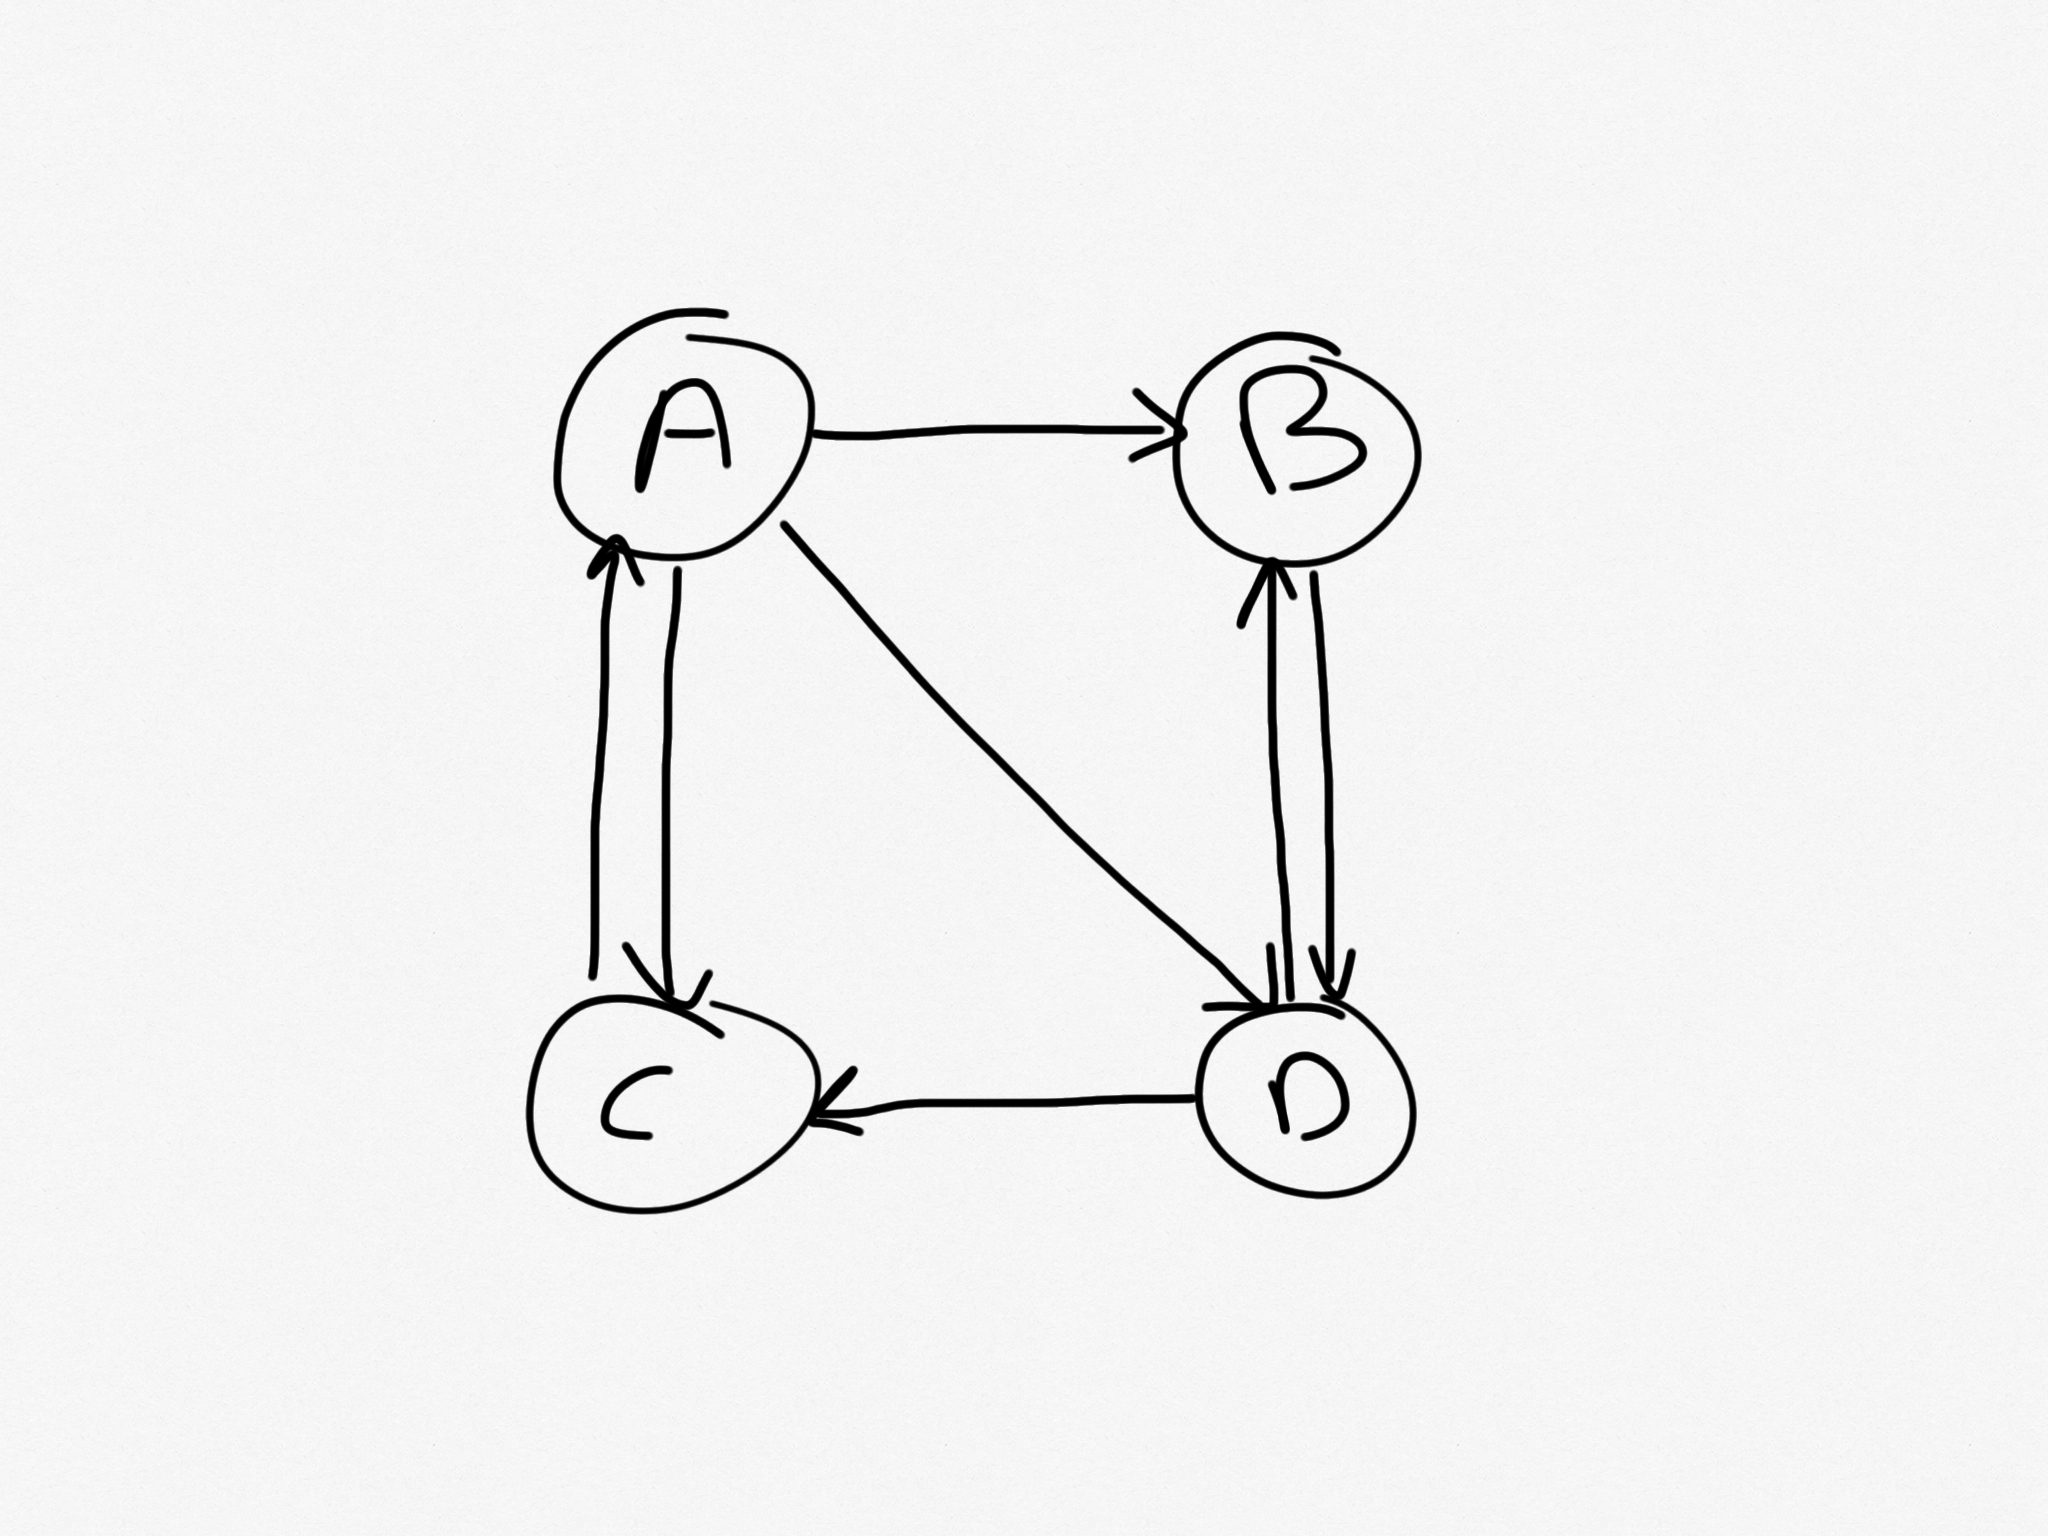
\includegraphics[width=0.9\textwidth]{graph1.PNG}
    \caption{The graph for question 1.1}
    \label{fig:g1}
\end{figure}


\end{document}